\section{Week 10 : CAP Theorem}

\subsection{CAP Theorem - Intro}
The CAP Theorem states that in a distributed system, you can only guarantee two out of the following three properties:

\begin{enumerate}[itemsep=1pt, topsep=1pt]
\item \textbf{Consistency (C):} Every read receives the most recent write or an error. All nodes see the same data at the same time.
\item \textbf{Availability (A):} Every request receives a (non-error) response, without the guarantee that it contains the most recent write.
\item \textbf{Partition Tolerance (P):} The system continues to operate despite an arbitrary number of messages being dropped (or delayed) by the network between nodes.
\end{enumerate}

\noindent The core idea is that when a network partition (a communication breakdown) occurs, you must choose between consistency and availability. You cannot have all three.

Rob G. references "Distributed systems for fun and profit on chapter 2", which has a helpful Venn diagram, as well as a link to the reading at book.mixu.net.

\subsubsection{CAP Theorem Combinations}
Because of the "choose two" nature, there are three primary system types:

\begin{enumerate}[itemsep=1pt, topsep=1pt]
\item \textbf{CA (Consistency and Availability):} These systems prioritize consistency and availability in the absence of network partitions. However, when a partition occurs, they may become unavailable to maintain consistency. Examples include traditional relational databases that do not account for partition tolerance, such as with a two-phase commit.
\item \textbf{CP (Consistency and Partition Tolerance):} These systems prioritize consistency even during network partitions. If a partition occurs, they may become unavailable on some nodes to ensure that data remains consistent across the accessible nodes.
\item \textbf{AP (Availability and Partition Tolerance):} These systems prioritize availability, even during network partitions. They will continue to serve requests, but some nodes might return stale or inconsistent data.
\end{enumerate}

\begin{figure}[h]
\begin{center}
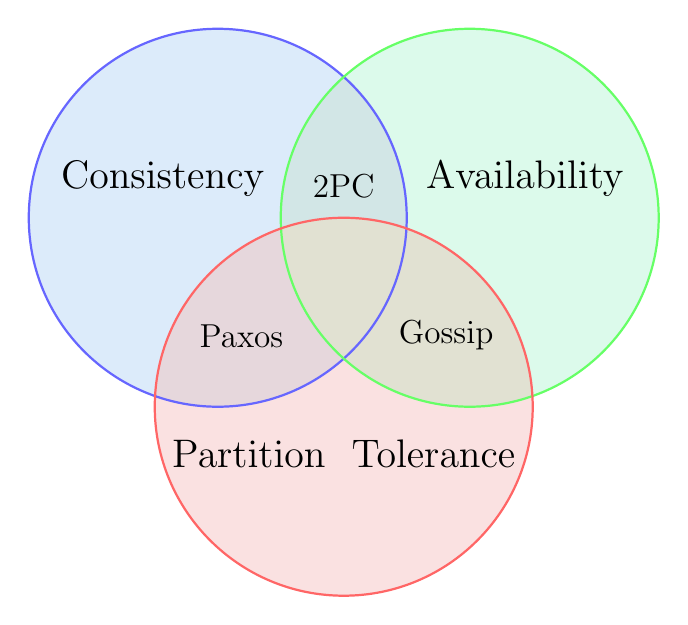
\begin{tikzpicture}
    % Define colors
    \definecolor{consistencyColor}{RGB}{220,235,250}
    \definecolor{availabilityColor}{RGB}{220,250,235}
    \definecolor{partitionColor}{RGB}{250,225,225}
    \definecolor{paxosColor}{RGB}{230,215,220}
    \definecolor{gossipColor}{RGB}{225,225,210}
    \definecolor{twopcColor}{RGB}{210,230,230}
    % Circle radius
    \def\R{2.4}
    % Draw filled circles
    \fill[consistencyColor] (-1.6,0) circle (\R);
    \fill[availabilityColor] (1.6,0) circle (\R);
    \fill[partitionColor] (0,-\R) circle (\R);
    % Intersection areas - fixed positions
    \begin{scope}
        \clip (-1.6,0) circle (\R);
        \clip (1.6,0) circle (\R);
        \fill[twopcColor] (0,0) circle (2*\R);
    \end{scope}
    \begin{scope}
        \clip (-1.6,0) circle (\R);
        \clip (0,-\R) circle (\R);
        \fill[paxosColor] (0,0) circle (2*\R);
    \end{scope}
    \begin{scope}
        \clip (1.6,0) circle (\R);
        \clip (0,-\R) circle (\R);
        \fill[gossipColor] (0,0) circle (2*\R);
    \end{scope}
    % Draw circle outlines
    \draw[thick, blue!60] (-1.6,0) circle (\R);
    \draw[thick, green!60] (1.6,0) circle (\R);
    \draw[thick, red!60] (0,-\R) circle (\R);
    % Labels for main circles (placed on circle edges)
    \node at (-2.3,0.5) {\Large Consistency};
    \node at (2.3,0.5) {\Large Availability};
    \node at (0,-3) {\Large Partition \ Tolerance};
    % Labels for intersections
    \node at (0,0.4) {\large 2PC};
    \node at (-1.3,-1.5) {\large Paxos};
    \node at (1.3,-1.5) {\large Gossip};
\end{tikzpicture}
\end{center}
\label{fig:cap_theorem}
\caption{CAP theorem Venn Diagram}
\end{figure}


\subsection{Two-Phase Commit (2PC) as a CA System}
In 2PC, there are $n$ nodes in a distributed database.

\begin{enumerate}[itemsep=0.5pt, topsep=1pt]
\item A coordinator node initiates a transaction by sending a \texttt{lock} request to all other $n-1$ nodes.
\item All $n-1$ nodes respond with \texttt{OK} to acknowledge the lock request.
\item The coordinator makes the change.
\item The coordinator sends a message, to all other nodes, to indicate that the change has been made.
\item All $n-1$ nodes respond with \texttt{OK} to aknowledge.
\end{enumerate}

\noindent This protocol ensures \textbf{strong consistency} because all nodes must agree before a change is committed   and the data is available. However, if any node fails or a network partition occurs, the entire system can become unavailable. The coordinator needs all of the responses.

\noindent This type of communication requires $4(n-1)$ messages in total.

\subsubsection{Partition Tolerance and Majority Rules}
Consider a system with five nodes. If a network partition splits the nodes into two groups (e.g., three in the USA and two in Asia), the group with the majority of nodes (three in this case, in the USA) can continue to operate and make changes.

The disconnected nodes (in Asia) become unavailable to maintain consistency. When the partition is resolved, the nodes can rejoin, and the data can be synchronized. This system chooses Consistency and Partition-tolerance, sacrificing availability on all nodes.


\subsection{Availability and Partition Tolerance (AP System)}
With an AP system, all partitions of nodes can continue to operate even in the face of a total partition. There is no lock, or strong consistency, so the changes that happen on a given side of the partition are not guarenteed to be the same changes that happen on another node.

When a merge of the partitions happen, there is no way to know which changes are \texttt{right}. The system continues to operate, but this may result in the nodes having conflicts, and stale or inconsistent data.


\subsubsection{A Note About Even-Numbered Partition Tolerance}
When making thought experiments of partitioning, it can be important to maintain an odd number of nodes for the sake of determining majority. With an even number of nodes, it can be impossible to determine, as two equal partitians are not a majority.

\subsection{Key Takeaways}

\begin{itemize}[itemsep=1pt, topsep=1pt]
\item The CAP Theorem states that you can only guarantee two of Consistency, Availability, and Partition Tolerance in a distributed system.
\item When a network partition occurs, you must choose between consistency and availability.
\item There is a strong tension between consistency and availability.
\item Different system designs (CA, CP, AP) make different trade-offs based on the application's requirements.
\end{itemize}

\endclass{Week 10}